\documentclass[12pt]{article}

\usepackage{answers}
\usepackage{setspace}
\usepackage{graphicx}
\usepackage{enumitem}
\usepackage{multicol}
\usepackage{mathrsfs}
\usepackage[margin=1in]{geometry} 
\usepackage{amsmath,amsthm,amssymb}
 
\newcommand{\N}{\mathbb{N}}
\newcommand{\Z}{\mathbb{Z}}
\newcommand{\C}{\mathbb{C}}
\newcommand{\R}{\mathbb{R}}

\DeclareMathOperator{\sech}{sech}
\DeclareMathOperator{\csch}{csch}
 
\newenvironment{theorem}[2][Theorem]{\begin{trivlist}
\item[\hskip \labelsep {\bfseries #1}\hskip \labelsep {\bfseries #2.}]}{\end{trivlist}}
\newenvironment{definition}[2][Definition]{\begin{trivlist}
\item[\hskip \labelsep {\bfseries #1}\hskip \labelsep {\bfseries #2.}]}{\end{trivlist}}
\newenvironment{proposition}[2][Proposition]{\begin{trivlist}
\item[\hskip \labelsep {\bfseries #1}\hskip \labelsep {\bfseries #2.}]}{\end{trivlist}}
\newenvironment{lemma}[2][Lemma]{\begin{trivlist}
\item[\hskip \labelsep {\bfseries #1}\hskip \labelsep {\bfseries #2.}]}{\end{trivlist}}
\newenvironment{exercise}[2][Exercise]{\begin{trivlist}
\item[\hskip \labelsep {\bfseries #1}\hskip \labelsep {\bfseries #2.}]}{\end{trivlist}}
\newenvironment{solution}[2][Solution]{\begin{trivlist}
\item[\hskip \labelsep {\bfseries #1}]}{\end{trivlist}}
\newenvironment{problem}[2][Problem]{\begin{trivlist}
\item[\hskip \labelsep {\bfseries #1}\hskip \labelsep {\bfseries #2.}]}{\end{trivlist}}
\newenvironment{question}[2][Question]{\begin{trivlist}
\item[\hskip \labelsep {\bfseries #1}\hskip \labelsep {\bfseries #2.}]}{\end{trivlist}}
\newenvironment{corollary}[2][Corollary]{\begin{trivlist}
\item[\hskip \labelsep {\bfseries #1}\hskip \labelsep {\bfseries #2.}]}{\end{trivlist}}
 
\begin{document}
 
% --------------------------------------------------------------
%                         Start here
% --------------------------------------------------------------
 
\title{Chaos and complexity assignment}%replace with the appropriate homework number
\author{Oisín Peppard - 16323022\\ %replace with your name
T.P.- JF Hilary} %if necessary, replace with your course title
 
\maketitle
%Below is an example of the problem environment

\begin{problem}{1}
The given equation of motion for a driven, damped oscillator is 
\begin{equation}
    \Ddot{\theta} + \frac{\dot{\theta}}{q} + \theta = 0
\end{equation}
The aim is to show that the Ansatz function 
\begin{equation}
    \theta(t) = e^{-\frac{1}{2q}t}\cos{rt}
\end{equation}
solves the ODE. To check this, we substitute and check manually.
\[\dot{\theta} = -\frac{1}{2q}e^{-\frac{1}{2q}t}\cos{rt} - re^{-\frac{1}{2q}t}\sin{rt}\]
\[\Ddot{\theta(t)} = \frac{1}{4q^2}e^{-\frac{1}{2q}t}\cos{rt} + \frac{r}{q}e^{-\frac{1}{2q}t}\sin{rt} - r^2e^{-\frac{1}{2q}t}\cos{rt}\]
By substituting back into equation (1), the ODE becomes 
\begin{equation}
    (1-r^2-\frac{1}{4q^2})e^{-\frac{1}{2q}t}\cos{rt} = 0
\end{equation}
This means the Ansatz works for the roots of the quadratic in $r$:
\[ 1-r^2-\frac{1}{4q^2} = 0\]

The same result can be obtained by employing the auxiliary equation method to solving this homogenous second order linear differential equation.
\[\lambda^2 + \frac{\lambda}{q} + \lambda = 0\]
Yielding 
\[\lambda = -\frac{1}{2q} \pm \sqrt{1-\frac{1}{4q^2}}\] 
and general complex solution 
\[\theta_c(t) = e^{-\frac{1}{2q}t}e^{irt}\]
and \[\Re(\theta_c) = \theta(t) = e^{-\frac{1}{2q}t}\cos{rt}\] 

\end{problem}

\begin{problem}{2}
Solving the quadratic from equation (3), one obtains
\[ r = \sqrt{1-\frac{1}{4q^2}}\]
This solution is real, and overdamping will occur if $q < \frac{1}{2}$. Critical damping if $q = \frac{1}{2}$ and underdamping if $q > \frac{1}{2}$
\end{problem}

\begin{problem}{3}

It can be seen here that for a value of $q = \frac{1}{2}$ the system is critically damped, and the oscillator will come to rest at exactly the end of its first oscillation. When $q > \frac{1}{2}$ the system is heavily damped and comes to rest quickly, however it is underdamped and completes some cycles before it does. For $q >> \frac{1}{2}$ the damping is far less effective and the system oscillates for longer before reaching the stable equilibrium. When $q$ was set to the comparatively large value of  100,000,000 the system appeared to be completely undamped and would oscillate indefinitely. However in reality, this too would eventually come to rest. Had the simulation run for longer this would be apparent in the phase portrait. Results are shown in Figure 1.





\end{problem}


\begin{problem}{4}
The aim here is to construct a numerical integration of phase space to produce the same portraits as the analytical method. We first need to derive differentials in $\theta$ and $\omega$. Given that 
\[\frac{\Delta\omega}{\Delta\theta}\approx \frac{d\omega}{\theta} = f(\theta, \omega)\] and
\[\delta^2 = (\Delta\theta)^2 + (\Delta\omega)^2\]
These can be combined to produce the following 
\[\frac{\delta^2}{(\Delta\theta)^2} = 1 + f^2\]
\[(\Delta\theta)^2 = \frac{\delta^2}{1+f}\]
\begin{equation}
\Delta\theta = \pm\frac{\delta}{\sqrt{1+f^2}}
\end{equation}
\[\Delta\omega = \frac{\Delta\omega}{\Delta\theta} \times \Delta\theta\]
\begin{equation}
    \Delta\omega = \pm \frac{f\delta}{\sqrt{1+f^2}}
\end{equation}

\end{problem}

\begin{problem}{5}
\[\frac{d\omega}{dt} + \frac{\omega}{q} + \theta = 0\]
can be manipulated to obtain $\frac{d\omega}{d\theta}$ as a function of $\theta, \omega,$ and $q$
\begin{equation}
    f(\omega, \theta) = -\frac{1}{q} - \frac{\theta}{\omega}
\end{equation}
Equations (4) and (5) are rewritten to resolve the ambivalence of $\pm$. 
\[\Delta\theta\ = \frac{\omega}{|\omega|}\frac{\delta}{\sqrt{1+f^2}}\]
\[\Delta\omega = f\Delta\theta\]

The above formulae are used to construct an iterative numerical function for each of $\theta$ and $\omega$. The following simple relations are employed
\[\theta_{n+1} = \theta_n + \Delta\theta\]
\[\omega_{n+1} = \omega_n + \Delta\theta\]
An appropriate python script is added and run to emulate the results of the analytic solution. The following results are obtained and displayed in Figure 2. The numerical method functions effectively for appropriate values of $\delta$ and sufficient number of iterations $N$. In the above examples, step size $\delta$ was set to 0.0001 and $N = 1000000$ iterations were run. The simulations in Figure 3 demonstrate the inaccuracy as a result of $\delta$ too large and/or $N$ too small.

\end{problem}

\begin{figure}
\centering
\begin{minipage}[t]{0.45\textwidth}
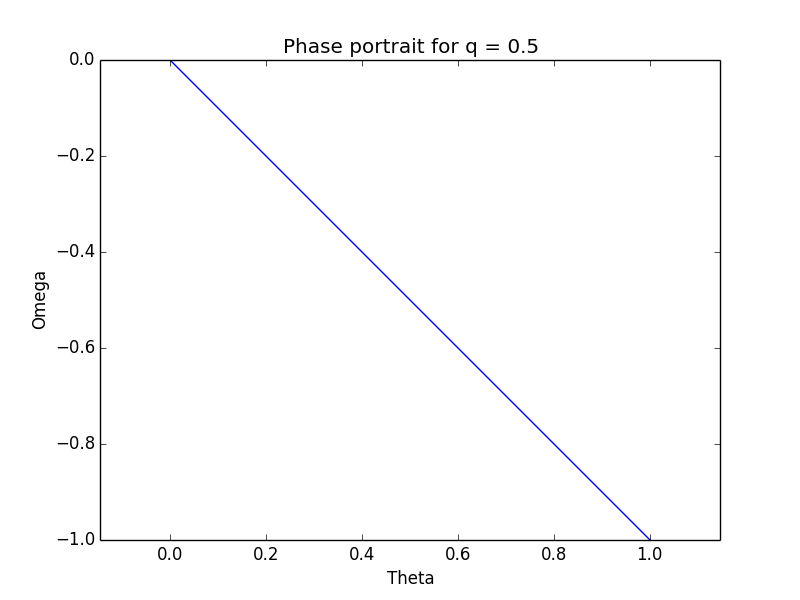
\includegraphics[width=\textwidth]{05.png}
\end{minipage}
\begin{minipage}[t]{0.45\textwidth}
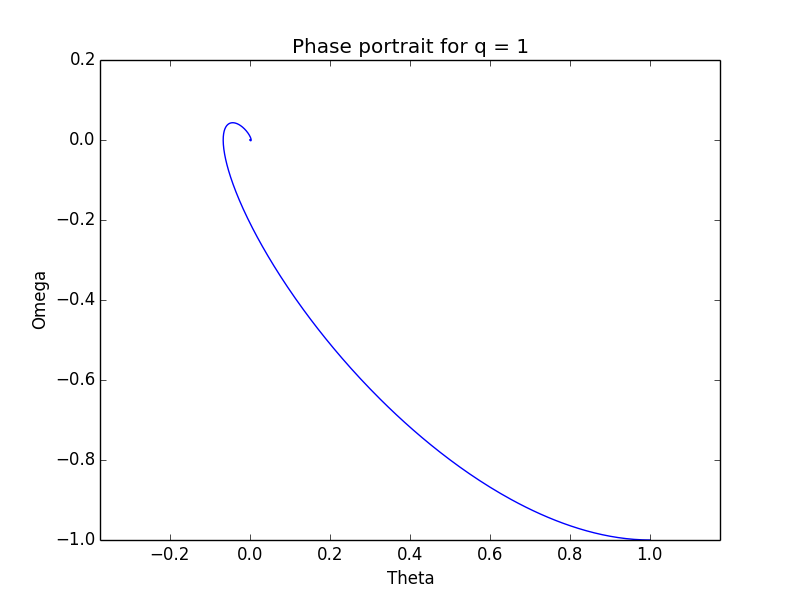
\includegraphics[width=\textwidth]{1.png}
\end{minipage}
\begin{minipage}[t]{0.45\textwidth}
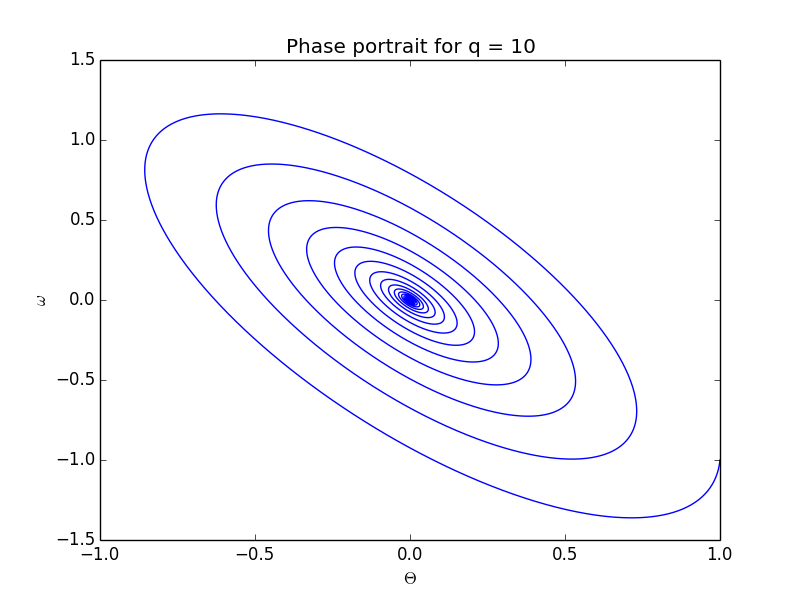
\includegraphics[width=\textwidth]{10.png}
\end{minipage}
\begin{minipage}[t]{0.45\textwidth}
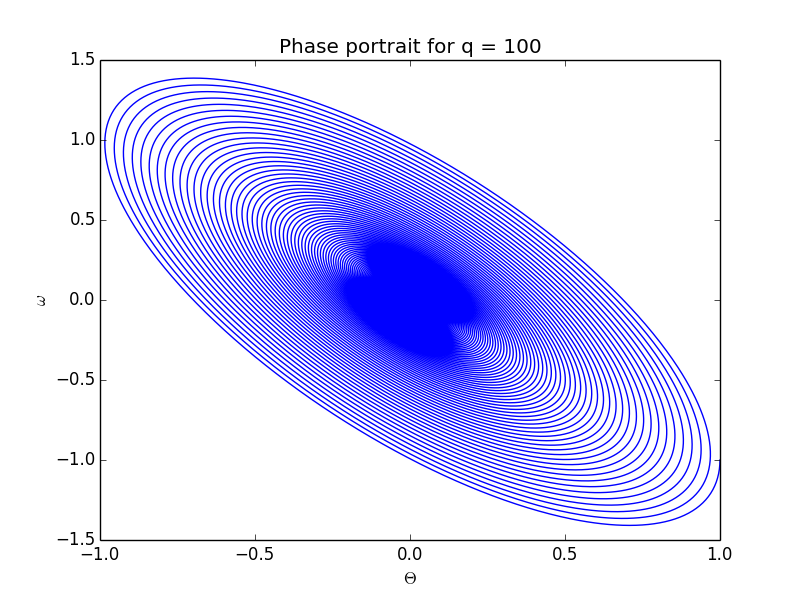
\includegraphics[width=\textwidth]{100.png}
\end{minipage}
\begin{minipage}[t]{0.45\textwidth}
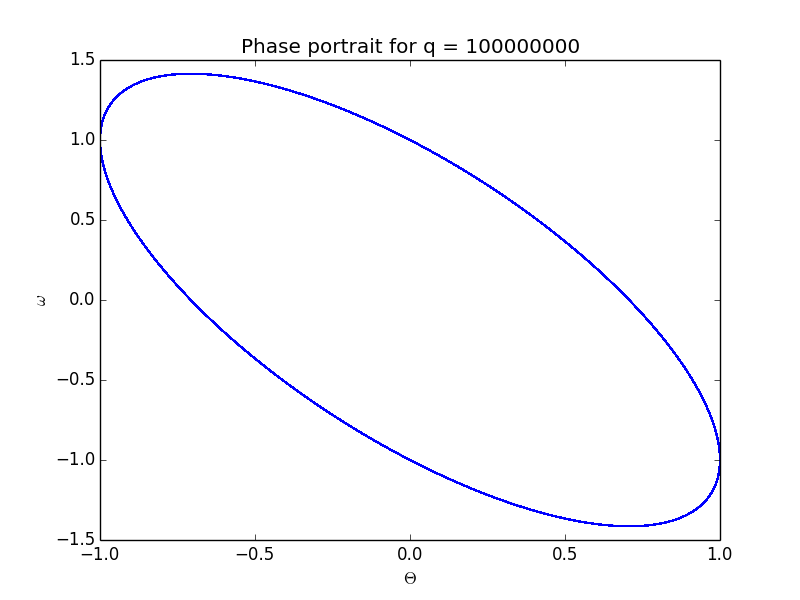
\includegraphics[width=\textwidth]{1000000.png}
\end{minipage}
\caption{Phase portraits for various damping coefficients $q$}
\label{fig:1}   
\end{figure}


\begin{figure}[]
\centering
\begin{minipage}[t]{0.45\textwidth}
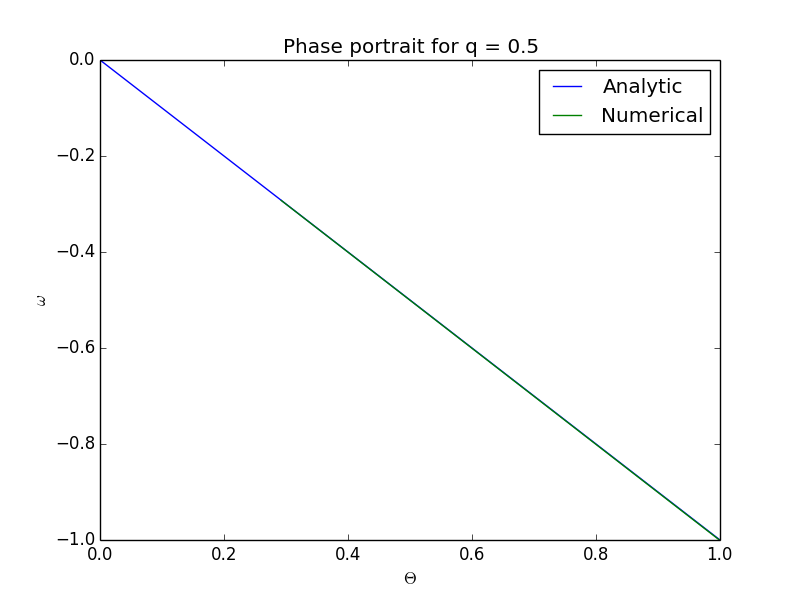
\includegraphics[width=\textwidth]{both05.png}
\end{minipage}
\begin{minipage}[t]{0.45\textwidth}
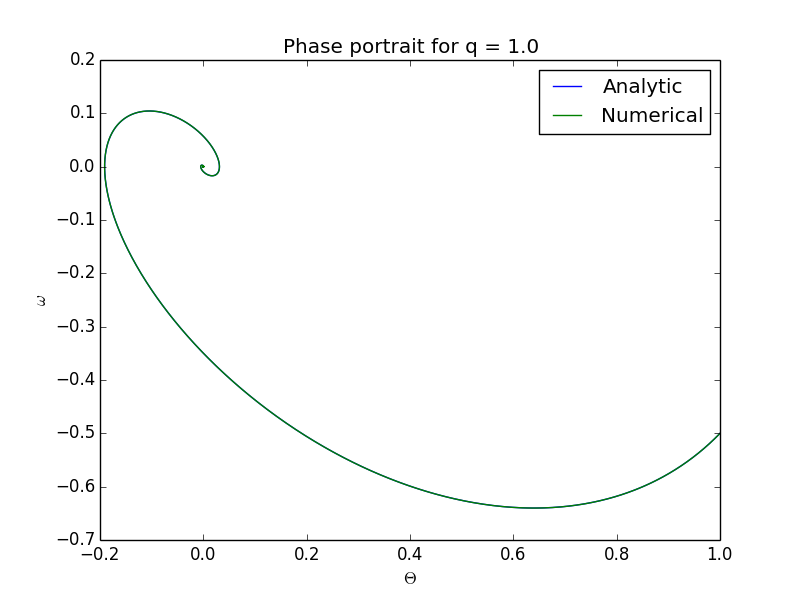
\includegraphics[width=\textwidth]{both1.png}
\end{minipage}
\begin{minipage}[t]{0.45\textwidth}
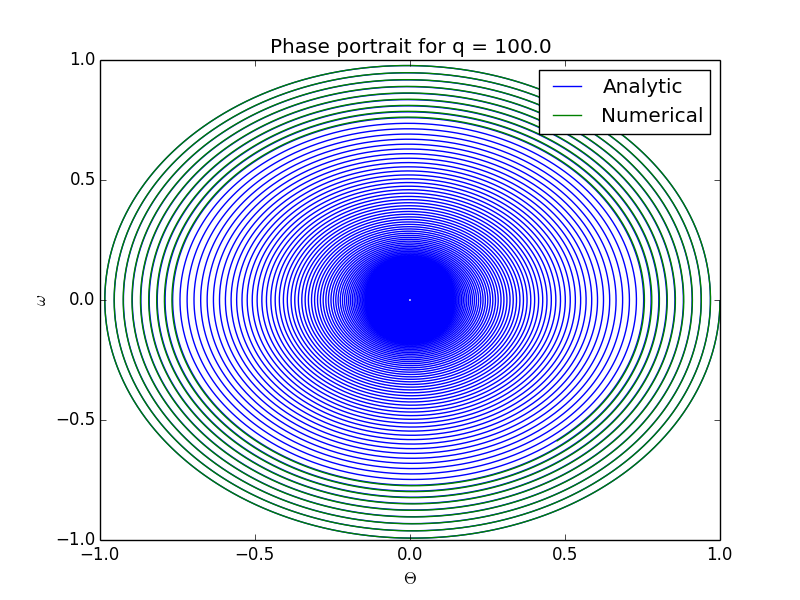
\includegraphics[width=\textwidth]{both100}
\end{minipage}
\begin{minipage}[t]{0.45\textwidth}
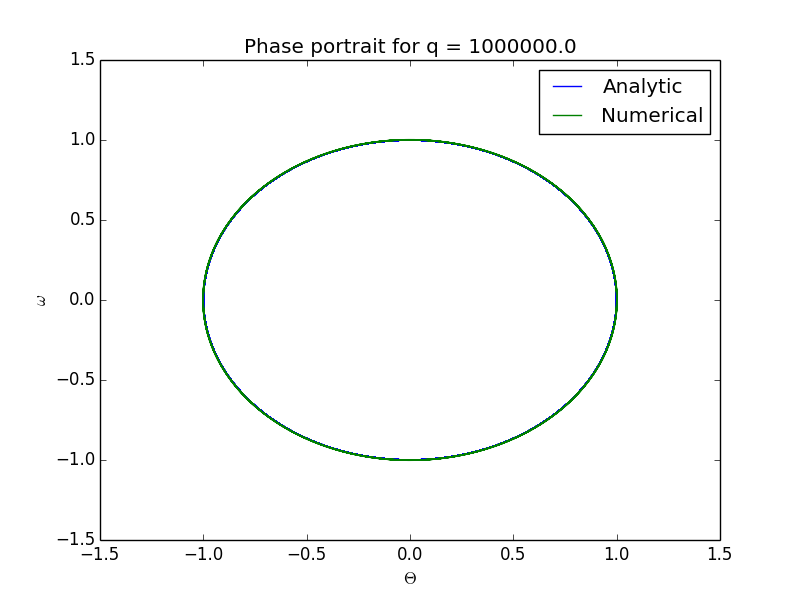
\includegraphics[width=\textwidth]{both10000000.png}
\end{minipage}
\caption{Phase portraits for various damping coefficients $q$, numerical and analytic computation}
\label{fig:2}   
\end{figure}



\begin{figure}[]
\centering
\begin{minipage}[t]{0.45\textwidth}
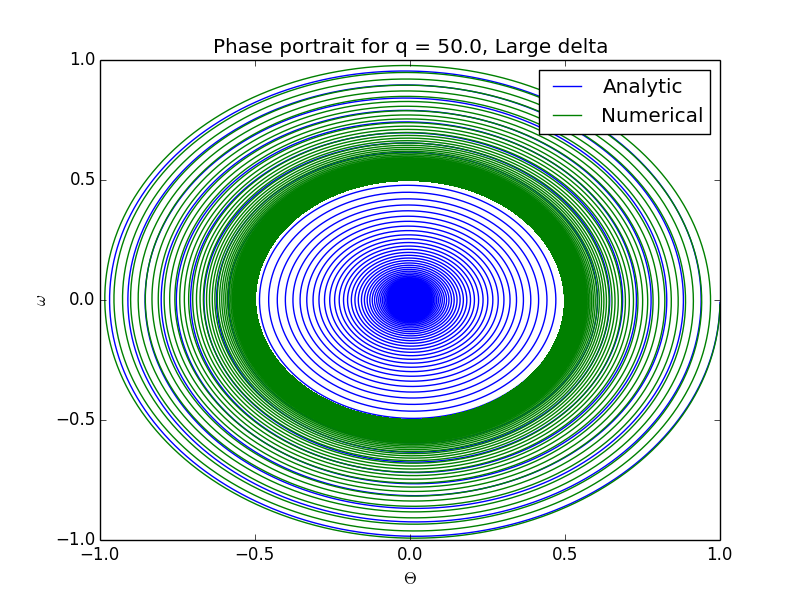
\includegraphics[width=\textwidth]{Largedelta.png}
\end{minipage}
\begin{minipage}[t]{0.45\textwidth}
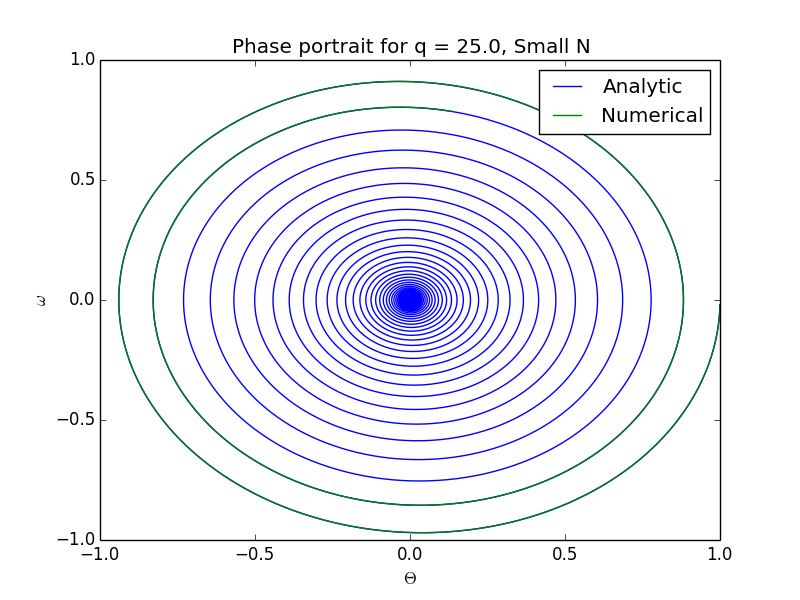
\includegraphics[width=\textwidth]{SmallN.png}
\end{minipage}
\caption{Dependency of appropriate $\delta$ and $N$}
\label{fig:3}   
\end{figure}

\end{document}
